\documentclass{article}

\usepackage{svg}
\usepackage{microtype}
\usepackage[framemethod=tikz]{mdframed}
\usepackage{hyperref}
\usepackage{url}
\usepackage{xspace}
\hypersetup{
    colorlinks,
    citecolor=black,
    filecolor=black,
    linkcolor=black,
    urlcolor=black
}
\usepackage{courier}
\usepackage{listings, xcolor}
\lstset{
    tabsize = 4,
    showstringspaces = false, 
    numbers = left,
    commentstyle = \color{green},
    keywordstyle = \color{blue},
    stringstyle = \color{red},
    rulecolor = \color{black},
    basicstyle = \small \ttfamily ,
    breaklines = true,
    numberstyle = \tiny,
}

\author{Elisa Zanella e Lorenzo Mioso}

\title{Documentazione progetto Ingegneria del Software}

\begin{document}

\maketitle

\newpage

\tableofcontents

\newpage

\listoffigures

\newpage

\section{Requisiti ed interazioni utente-sistema}

\subsection{Specifiche casi d’uso}

Il sistema è diviso in due parti principali. Una dedicata all'utente e l'altra
al responsabile del reparto. Per \textbf{utente} si intende la persona che utlilizza questo
servizio per fare la spesa e per \textbf{responsabile reparto} l'impiegato che gestisce
il reparto a lui assegnato. L’utente non necessita di autenticarsi per consultare il
catalogo dei prodotti, ma per acquistarli deve registrarsi nel sistema, invece il
responsabile deve autenticarsi con delle credenziali pre-fornite dagli amministratori
del sistema.

\subsubsection{Casi d'uso relativi all'utente}

\begin{figure}[h!]
	\centering
	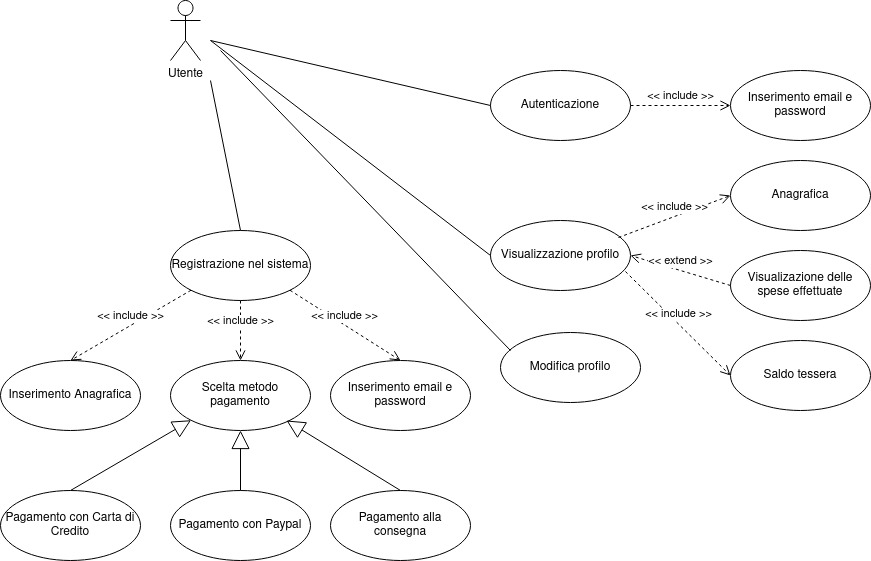
\includegraphics[width=\textwidth]{UseCaseUtenteGestioneProfilo.jpg}
	\caption{Use case di utente per la gestione del profilo e la registrazione}
	\label{fig:UseCaseUtenteGestioneProfilo}
\end{figure}

\newpage


\paragraph{Registrazione nel sistema:}

\begin{mdframed}

	\noindent\textit{\textbf{Attori :}}


	Utente

	\noindent\textit{\textbf{Descrizione :}}


	Procedura di inserimento dei dati dell’utente per registrarsi nel
	sistema

	\noindent\textit{\textbf{Sequenza di eventi :}}


	L’utente inserisce i suoi dati relativi all'anagrafica,
	scelta di metodo di pagamento preferito, email e password.

	\noindent\textit{\textbf{Post condizioni:}}


	Il sistema registra l’utente con i dati inseriti

	\noindent\textit{\textbf{Sequenza Alternativa :}}


	Se i dati inseriti non sono validi il sistema non effettua la
	registrazione
	Se l'email è già stata inserita nel sistema,
	il sistema ne richiede una diversa
\end{mdframed}

\begin{figure}[h!]
	\centering
	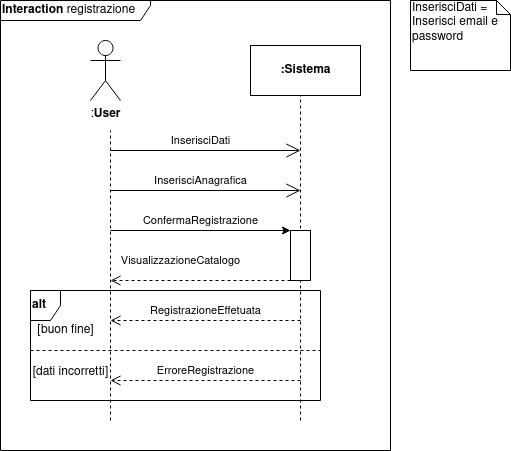
\includegraphics[width=\textwidth]{SDregistrazione.jpg}
	\caption{Sequence Diagram della registrazione}
	\label{fig:SDregistrazione}
\end{figure}
\newpage
\paragraph{Autenticazione:}
\begin{mdframed}

	\noindent\textit{\textbf{Attori :}}


	Utente

	\noindent\textit{\textbf{Descrizione :}}


	Procedura di autenticazione dell'utente

	\noindent\textit{\textbf{Sequenza di eventi :}}


	L’utente inserisce i dati necessari per l'autenticazione

	\noindent\textit{\textbf{Pre-condizioni:}}


	L'utente deve essere registrato nel sistema

	\noindent\textit{\textbf{Sequenza Alternativa :}}


	Se i dati inseriti non sono validi il sistema non effettua
	l'autenticazione

\end{mdframed}

\begin{figure}[h!]
	\centering
	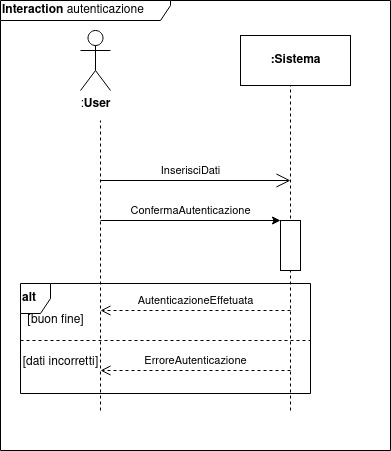
\includegraphics[width=\textwidth]{SDautenticazione.jpg}
	\caption{Sequence Diagram dell'autenticazione}
	\label{fig:SDautenticazione}
\end{figure}

\newpage

\paragraph{Visualizzazione catalogo:}

\begin{mdframed}
	\noindent\textit{\textbf{Attori :}}


	Utente

	\noindent\textit{\textbf{Descrizione :}}


	Il sistema permette di visualizzare tutti i prodotti disponibili, e ordinarli:
	\begin{enumerate}
		\item in modo crescente e decrescente per prezzo
		\item in ordine alfabetico per marca (dalla A alla Z e dalla Z alla A)
	\end{enumerate}

	\noindent\textit{\textbf{Sequenza di eventi :}}


	L’utente accede all'area dedicata

\end{mdframed}

\paragraph{Gestione profilo:}

\begin{mdframed}
	\noindent\textit{\textbf{Attori:}}


	Utente


	\noindent\textit{\textbf{Scopo e Descrizione sintetica:}}


	Il sistema permette all'utente di gestire il proprio profilo.
	L’utente può visualizzare e modificare il proprio profilo.

	\noindent\textit{\textbf{Sequenza di eventi :}}

	Questo caso d’uso viene attivato quando l’utente vuole modificare o visualizzare il proprio profilo.
	\begin{enumerate}
		\item L’utente sceglie la funzione richiesta
		\item Uno dei seguenti casi d’uso viene utilizzato:
		      \begin{enumerate}
			      \item{ Modifica profilo:
			            comprende la modifica dell'anagrafica.}
			      \item{Visualizzazione profilo: comprende la visualizzazione\\dell'anagrafica,
			            delle spese effettuate e l'attuale saldo punti della tessera.}
		      \end{enumerate}
	\end{enumerate}

	\noindent\textit{\textbf{Pre condizioni:}}


	L’utente deve essere registrato ed aver fatto il login 	nel sistema

	\noindent\textit{\textbf{Post-condizioni:}}


	Se le operazioni di modifica vanno a buon fine lo stato del profilo viene modificato,
	altrimenti il profilo rimane invariato.

	\noindent\textit{\textbf{Sequenza Alternativa:}}


	Se i dati inseriti non sono validi il sistema non effettua modifiche.
\end{mdframed}
\newpage

\subsubsection{Gestione carrello:}

\begin{figure}[h!]
	\centering
	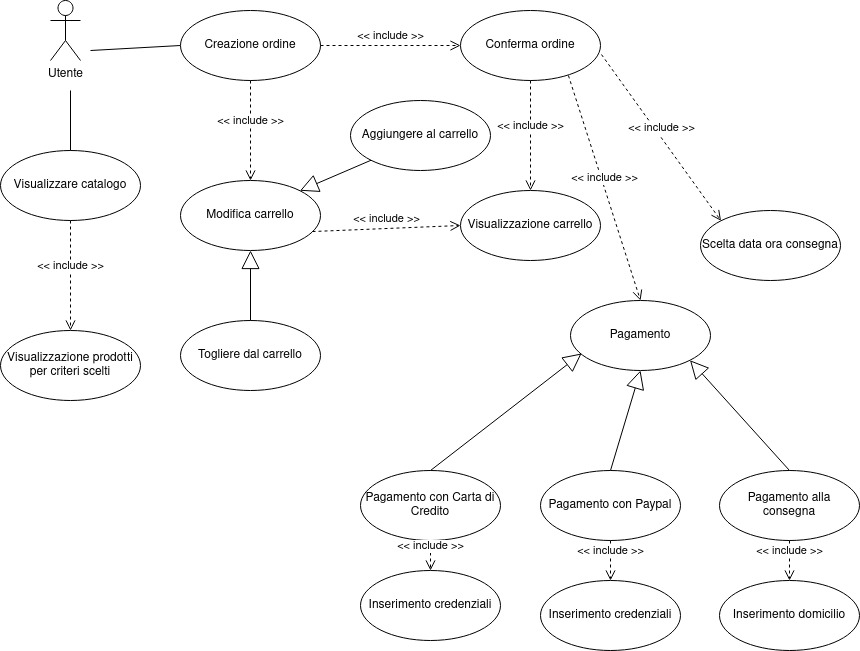
\includegraphics[width=\textwidth]{UseCaseUtenteGestioneCarrello.jpg}
	\caption{Use case del carrello}
	\label{fig:UseCaseUtenteGestioneCarrello}
\end{figure}

\newpage
\begin{mdframed}

	\noindent\textit{\textbf{Attori :}}


	Utente

	\noindent\textit{\textbf{Scopo e Descrizione sintetica :}}


	Il sistema permette all'utente di gestire il proprio carrello della spesa.
	L’utente può visualizzare il proprio carrello,
	inserire prodotti e togliere i prodotti già inseriti e confermare l’ordine. 

	\noindent\textit{\textbf{Sequenza di eventi :}}


	\hspace{\parindent} Questo caso d’uso viene attivato quando l’utente vuole modificare il proprio carrello.
	\begin{enumerate}
		\item L’utente sceglie la funzione richiesta
		\item Uno dei seguenti casi d’uso viene utilizzato:
		      \begin{enumerate}
			      \item Modifica al carrello(aggiungere e togliere prodotti)
			      \item Visualizzazione carrello
			      \item Conferma ordine:
			            Viene richiesta la data, l'ora di inizio e  di fine in cui può avvenire la consegna della spesa.
			            Il metodo di pagamento utilizzato per effettuare la spesa è quello scelto dall'utente durante la fase di registrazione o di modifica del profilo.
		      \end{enumerate}
	\end{enumerate}

	\noindent\textit{\textbf{Pre condizioni:}}


	L’utente deve essere registrato ed aver fatto il login 	nel sistema

	\noindent\textit{\textbf{Post-condizioni:}}


	Se le operazioni di modifica vanno a buon fine lo stato del carrello viene modificato,
	altrimenti il contenuto del carrello rimane invariato.
	Se la scelta della data e orario di consegna vanno a buon fine l’acquisto viene fatto, altrimenti l’acquisto
	non viene effettuato.

	\noindent\textit{\textbf{Sequenza Alternativa :}}


	Se durante la conferma il prodotto non è disponibile, viene visualizzato un
	messaggio di errore per informare l’utente che il prodotto non è disponibile.
	Se i dati inseriti non sono validi il sistema non effettua modifiche.
\end{mdframed}
\newpage
\begin{figure}[h!]
	\centering
	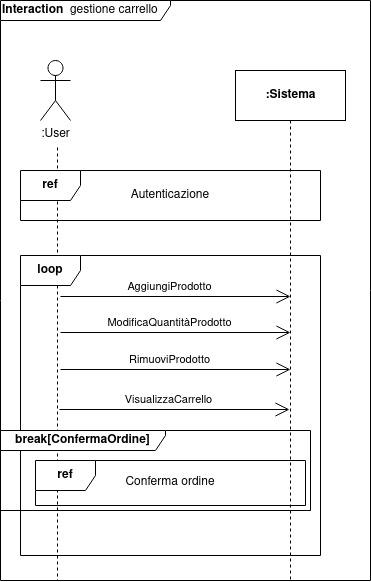
\includegraphics[width=\textwidth]{SDGestioneCarrello.jpg}
	\caption{Sequence Diagramm della gestione del carrello}
	\label{fig:SDGestioneCarrello}
\end{figure}

\begin{figure}[h!]
	\centering
	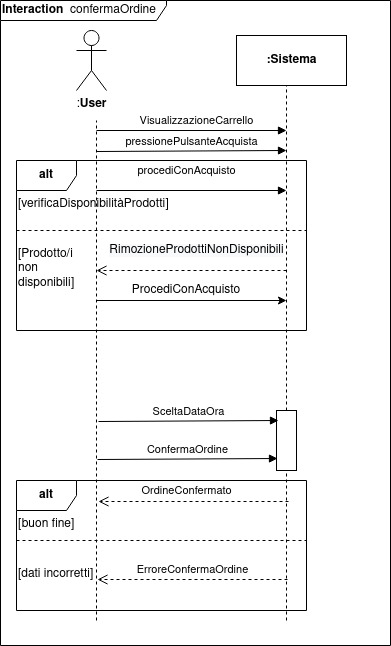
\includegraphics[width=\textwidth]{SDConfermaOrdine.jpg}
	\caption{Sequence Diagramm della conferma dell'ordine}
	\label{fig:SDConfermaOrdine}
\end{figure}
\newpage
\clearpage
\subsubsection{Casi d'uso relativi al responsabile reparto}

\begin{figure}[h!]
	\centering
	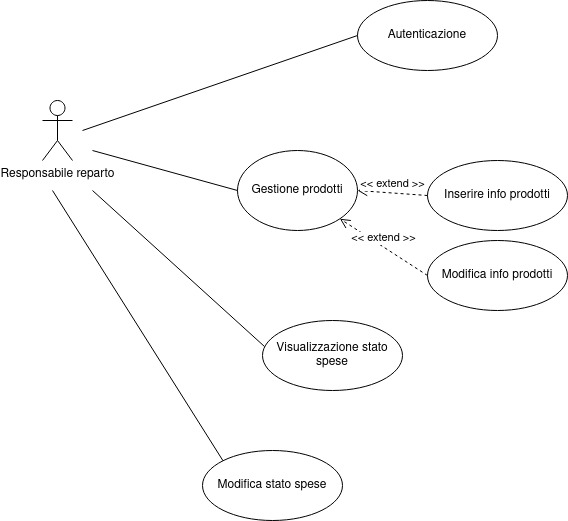
\includegraphics[width=\textwidth]{UseCaseResponsabile.jpg}
	\caption{Use case di responsabile reparto per l'autenticazione la gestione delle spese e dei prodotti}
	\label{fig:UseCaseResponsabile}
\end{figure}

\paragraph{Autenticazione:}
\begin{mdframed}

	\noindent\textit{\textbf{Attori :}}


	Responsabile reparto

	\noindent\textit{\textbf{Descrizione :}}


	Procedura di autenticazione del responsabile di reparto

	\noindent\textit{\textbf{Sequenza di eventi :}}


	Il responsabile inserisce i dati necessari per l'autenticazione

	\noindent\textit{\textbf{Pre-condizioni:}}


	Il responsabile deve essere presente nel sistema

	\noindent\textit{\textbf{Sequenza Alternativa :}}


	Se i dati inseriti non sono validi il sistema non effettua
	l'autenticazione

\end{mdframed}

\paragraph{Visualizzazione stato spese:}
\begin{mdframed}

	\noindent\textit{\textbf{Attori :}}


	Responsabile reparto

	\noindent\textit{\textbf{Descrizione :}}


	Sono visualizzati i dati relativi alle spese dei clienti.

	\noindent\textit{\textbf{Sequenza di eventi :}}


	Il responsabile accede all'area dedicata

	\noindent\textit{\textbf{Pre-condizioni:}}


	Il responsabile di reparto aver fatto il login nel sistema


	\noindent\textit{\textbf{Sequenza alternativa:}}


	Se i dati inseriti non sono validi il sistema non effettua modifiche

\end{mdframed}

\paragraph{Gestione prodotti}

\begin{mdframed}

	\noindent\textit{\textbf{Attori :}}


	Responsabile reparto

	\noindent\textit{\textbf{Descrizione :}}


	Il sistema permette al responsabile di gestire i prodotti del proprio reparto
	Con la possibilità di modificare e aggiungere i prodotti che sono terminati o che stanno
	per terminare.
	Inoltre può inserire nel sistema nuovi prodotti che appariranno sul catalogo 

	\noindent\textit{\textbf{Sequenza di eventi :}}


	Il responsabile accede all'area dedicata

	\noindent\textit{\textbf{Pre-condizioni:}}

	Il responsabile di reparto aver fatto il login nel sistema

	\noindent\textit{\textbf{Sequenza alternativa:}}


	Se i dati inseriti non sono validi il sistema non effettua modifiche
\end{mdframed}

\newpage
\section{Sviluppo: progetto dell'architettura ed implementazione del sistema}
\subsection{Note sul processo di sviluppo}
Precedentemente allo sviluppo si è cercato di trovare quanti più possibili pattern si potevano adattare al nostro progetto e si è valutata la scelta delle tecnologie da utilizzare man mano che si procedeva con lo sviluppo.

La fase di sviluppo ha previsto l'uso di molte tecnologie e metodologie di sviluppo che ci hanno permesso di poter ampliare ulteriormente le nostre competenze.
Da notare è il fatto che questi strumenti hanno richiesto un approfondimento da parte degli sviluppatori per poterli sfruttare al meglio e questo è stato possibile anche grazie a tutorial ed esempi online. Come nel caso dell'uso di JavaFX, di Git e GitHub.

\subsubsection{Metodologie di sviluppo}
Lo sviluppo è stato fatto completamente da remoto utilizzando sistemi di connessione come Skype e Discord. 

L'approccio principale di progettazione e sviluppo è basato sul modello agile, in cui ci sono stati dei macro cicli dove venivano progettate, implementate e testate funzionalità consistenti del prototipo. 
 Infatti per lo sviluppo del codice sono state adottate tecniche di pair-programming cercando di alternare e scambiare il più possibile il ruolo di navigator e di driver.

Il software è stato composto a partire dalla parte di sviluppo delle tabelle nel database utilizzando un progetto di supporto chiamato initDb per creare le tabelle e inizializzarle con dei dati. Successivamente si è passati a sviluppare la parte di Model in Java che comprende le classi che rappresentano i dati a cui sono associate le tabelle nel database e le classi DaoImpl dove ci sono le interrogazioni al database.  
In seguito si è svolta la parte di progettazione delle interfacce grafiche nella quale sono state adottate le tecniche di pair-designing facendo prima delle bozze intermedie e pianificando insieme come doveva essere il risultato finale.
Poi si è passati alla creazione di file fxml che rappresentavano le varie interfacce definite in precedenza. In contemporanea si sono sviluppate le corrispondenti classi Controller per mettere in comunicazione il Model con la View.

Durante lo sviluppo si è utilizzato Trello come piattaforma per fissare le attività da svolgere. Queste attività comprendevano fix di bug incontrati durante lo sviluppo e l'implementazione delle funzionalità richieste. 
\subsubsection{Tecnologie per lo sviluppo}
Durante lo sviluppo del software sono state utilizzate le seguenti tecnologie:
\begin{itemize}
    \item{\textbf{Netbeans}: per scrittura e compilazione del codice.}
    \item{\textbf{Maven}: per la gestione e sincronizzazione delle librerie.}
    \item{\textbf{SceneBuilder}: per la realizzazione delle interfaccie grafiche.}
    \item{\textbf{Git}: come strumento di controllo di versione a livello locale che si sincronizzava da remoto con github. }
    \item{\textbf{GitHub}: come servizio di hosting del codice. Infatti tutti i file necessari per lo sviluppo e la documentazione del progetto sono stati salvati all'interno di un unico repository condiviso.}
    \item{\textbf{MariaDB}: come sistema della gestione del database.}
    \item{\textbf{PhpMyAdmin}: come strumento di supporto per visualizzare il database durante lo sviluppo.}
    \item{\textbf{Latex}: per scrivere la documentazione. Inoltre è stato utilizzato Overleaf come strumento di condivisione e modifica live del codice Latex}

    \item{\textbf{draw.io}: per disegnare  i grafici (come use case, sequence diagram e activity diagram) online. }
    \item{\textbf{EasyUml}: un plug-in di NetBeans per generare l'UML}
\end{itemize}

\subsection{Progettazione e pattern architetturali usati}
Di seguito sono riportati tutti i pattern architetturali utilizzati 
\subsubsection{Pattern MVC}
Il progetto è strutturato con il Pattern MVC, perché fornisce una coerenza strutturale solida 
semplificando le fasi di progettazione e implementazione. Inoltre crea un'ottima sinergia con la
piattaforma JavaFX.

\noindent Il sistema è suddiviso in tre parti:
\begin{itemize}
    \item{\textbf{Model:}
            Sono presenti le classi che definiscono i dati manipolati
            e implementano la logica business.
            Inoltre sono presenti le classi che permettono la comunicazione
            con il Database organizzate seguendo il DAO pattern.
        }
    \item{\textbf{View:}
            Parte esclusivamente dedicata alla visualizzazione dei dati
            presenti nel modello.
            In particolare si utilizzano file del formato fxml per rappesentare
            l'interfaccia grafica.
        }
    \item{\textbf{Controller:}
            Le classi controller sono utilizzate come mezzo di comunicazione
            tra il Model e la View, permettono l'interazione dell'utente con il
            sistema e implementano della logica per validare i dati inseriti dall'utente.
        }
\end{itemize}
\subsubsection{Pattern Repository}
\noindent La memorizzazione dei dati avviene attraverso l'utilizzo di un database centrale chiamato Spesa nella quale è stata creata una tabella per ciascuna classe che implementa il DAO pattern. 

Le motivazioni che hanno portato alla scelta del repository pattern sono la semplicità d'uso e la centralità del sistema di recupero delle informazioni infatti è necessaria una sola classe per creare la connessione con il database ed eseguire le query (vedi classe ConnectionDb). 
\subsection{Note su JavaFX}
L'implementazione dell'interfaccia grafica è stata fatta utilizzano file fxml costruiti con SceneBuilder.
Questo permette di comporre in modularmene l'interfaccia grafica.
In varie parti del progetto si utilizza una vista che viene richiamata più volte per generare un contenuto
dinamico all'interno di una vista più complessa.(Es. Vedi Catalogo, contiene più istanze di un Prodotto)
\subsubsection{CSS}
JavaFX permette di utilizzare file .css per modificare l'aspetto dei componenti grafici.
Per migliorare l'estetica dell'applicativo é stato utilizzato un tema bootstrap chiamato jbootx.
\subsection{Implementazione e design pattern usati}
\newpage
\subsubsection{Pattern Sigleton}
Il pattern singleton è stato utilizzato nell'implementazione della classe ConnectionDb, allo scopo di
instaurare una connessione con il database, eseguire interrogazioni generiche e recuperare i risultati.
L'oggetto connectionDb viene istanziato una volta all'avvio dell'applicativo e viene utilizzato
da tutte le classi DaoImpl contenti le interrogazioni effettive.
\begin{figure}[h!]
	\centering
	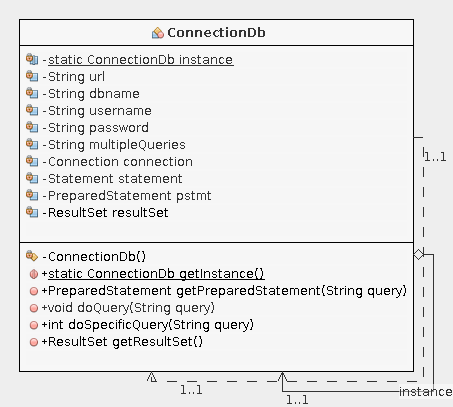
\includegraphics[width=\textwidth]{UmlConnectionDb.png}
	\caption{UML della classe ConnectionDb}
	\label{fig:UmlProdotto}
\end{figure}
\newpage

\subsubsection{Pattern Observer e gestione della sessione}
Durante lo sviluppo si è presentata la necessita di terner traccia dello stato di alcune istanze di oggetti che
sono visualizzati o modificati in più viste.
Per esempio se aggiungiamo al carrello un prodotto nel catalogo ci aspettiamo che la lista di prodotti nel
carrello sia aggiornata inserendo il prodotto scelto.
Per risolvere il problema di un'istanza di un oggetto condivisa tra più viste utilizziamo la classe SessionStorage
alla quale si è applicato il pattern Subject-Observer per notificare il cambiamento di stato.


\noindent Quindi la classe \textbf{SessionStorage} svolge il ruolo di \textbf{Subject} che notifica agli
Observer il cambiamento del suo stato.


\noindent Le classi \textbf{Controller} hanno il ruolo di \textbf{Observer} ad aggiornano la vista quando
il Subject cambia stato.

\begin{figure}[h!]
	\centering
	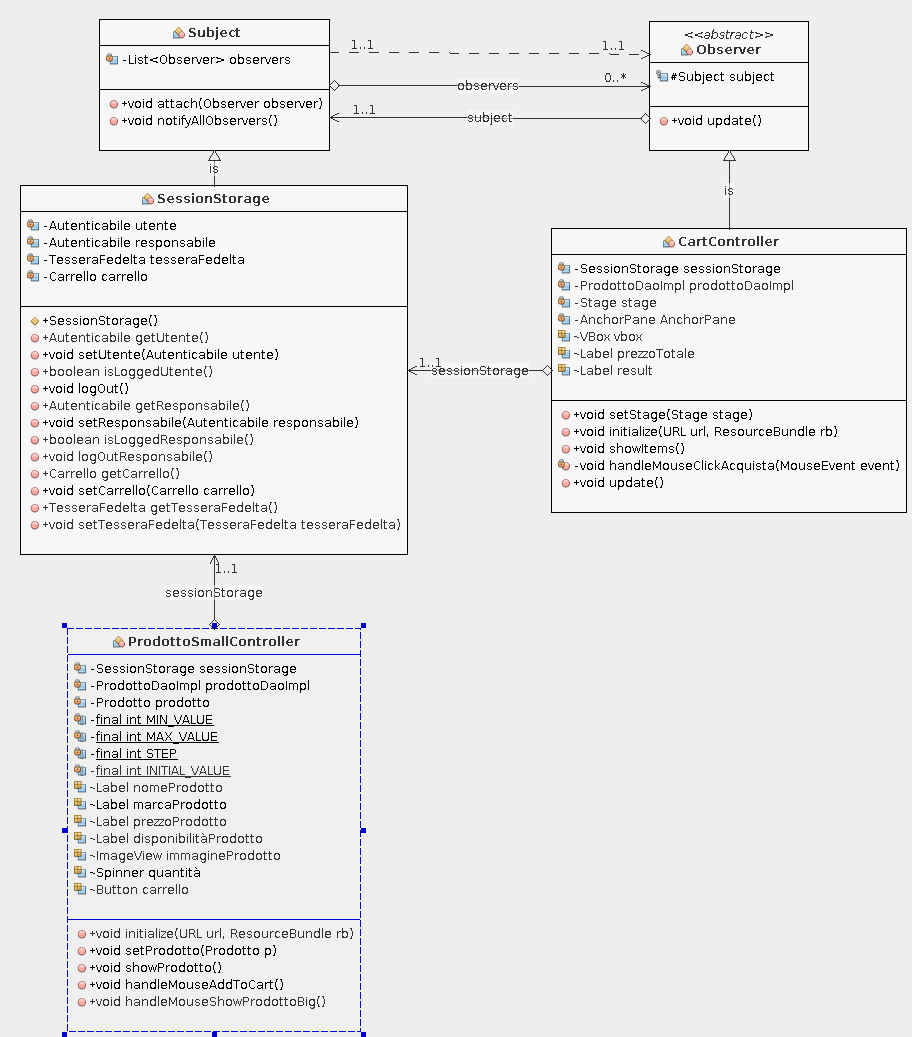
\includegraphics[width=\textwidth]{UmlObserver.png}
	\caption{UML delle classi che utilizzano il pattern Observer}
	\label{fig:UmlObserver}
\end{figure}
\clearpage
\newpage
\subsubsection{Pattern Data Access Object}
\'E stato utilizzato il DAO pattern per garantire accesso standardizzato alle risorse presenti nel database
tramite l'utilizzo di interrogazioni SQL.
Ogni oggetto nel package Model corrisponde a una tabella nel database e contiene metodi per reperire, inserire
e modificare le ennuple contenute nella tabelle.


\noindent La seguenti classi utilizzano il pattern DAO:
\begin{itemize}
	\item Caratteristica
	\item Prodotto
	\item Reparto
	\item ResponsabileReparto
	\item Spesa
	\item TesseraFedeltà
	\item Tipo
	\item Utente
\end{itemize}

\begin{figure}[h!]
	\centering
	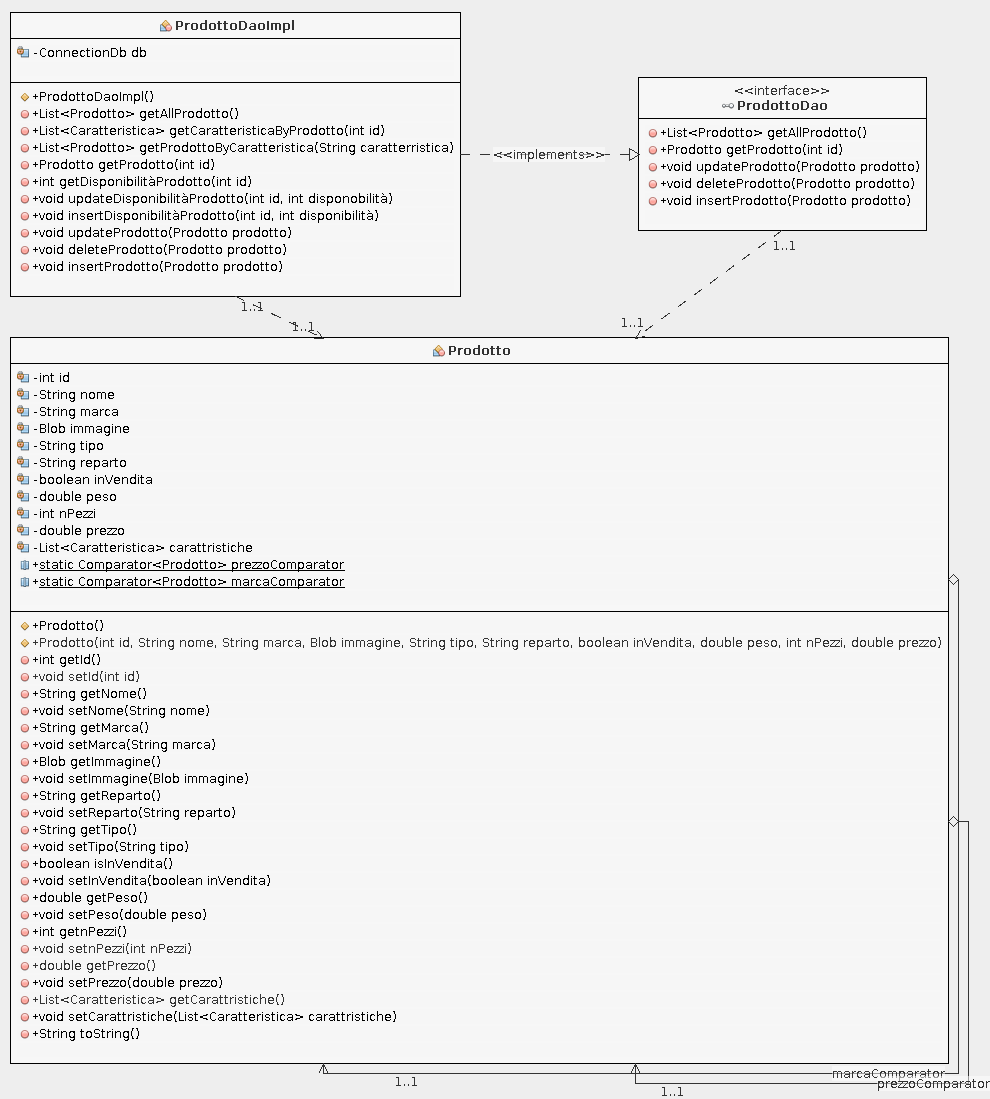
\includegraphics[width=\textwidth]{UmlProdotto.png}
	\caption{UML della classe Prodotto con pattern DAO}
	\label{fig:UmlProdotto}
\end{figure}
\clearpage
\subsubsection{UML delle Classi}
Di seguito sono riportati i relativi diagrammi delle classi della parte di Model, sono stati suddivisi in diverse immagini per poter facilitarne la visione (non sono presenti tutte le classi perché alcune sono state già inserite in precedenza nei pattern e l'implementazione DAO è stata messa quella di Prodotto per essere esempificativa a tutte le altre).
\begin{figure}[h!]
	\centering
	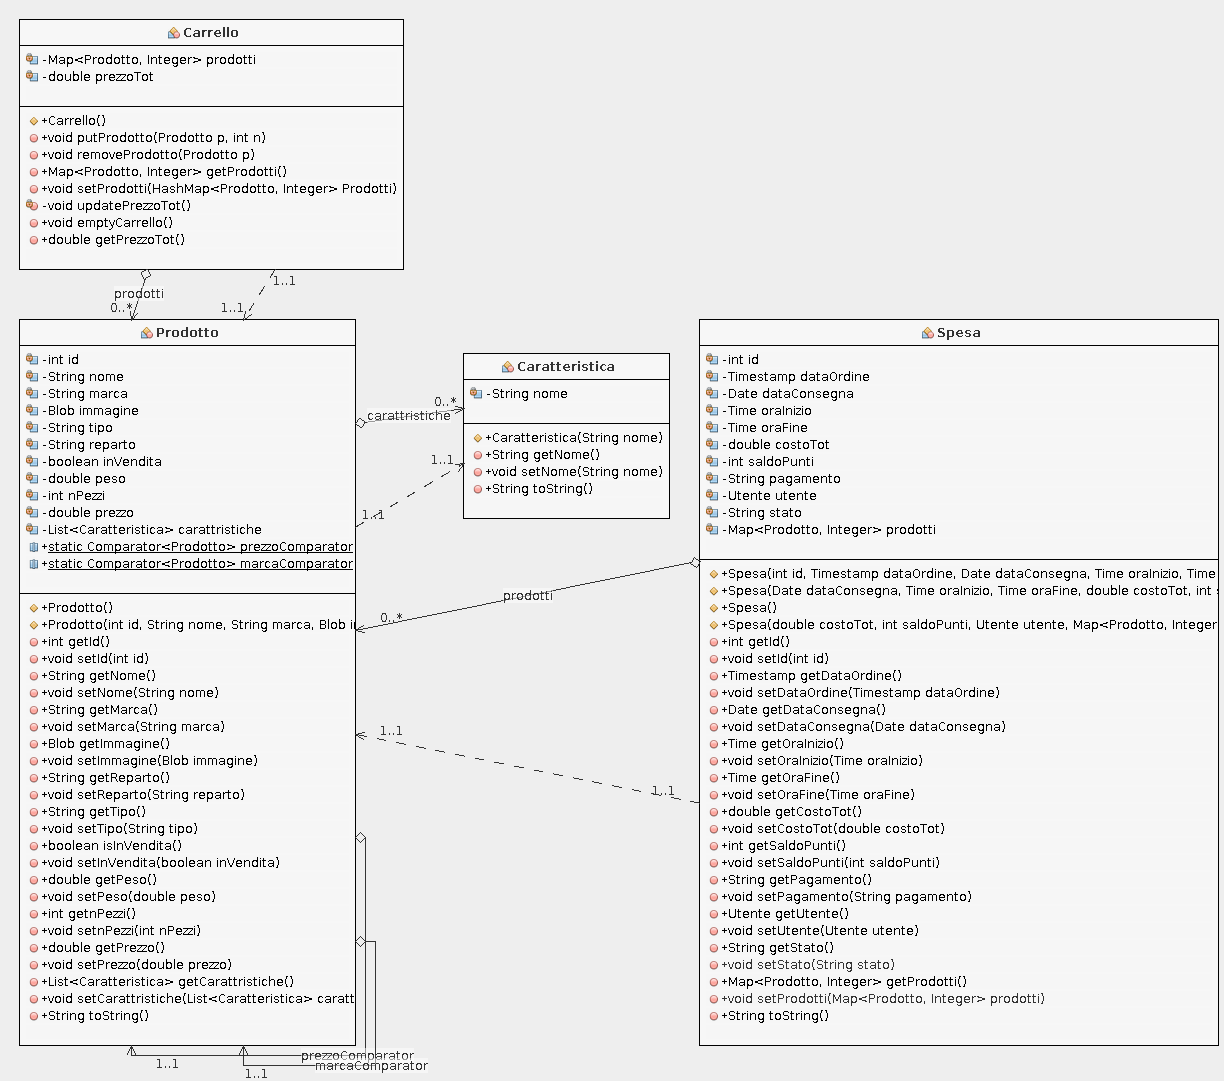
\includegraphics[width=\textwidth]{UmlSpesa.png}
	\caption{UML della classe Spesa e Carrello in relazione con Prodotto presenti nel model.}
	\label{fig:UmlSpesa}
\end{figure}
\begin{figure}[h!]
	\centering
	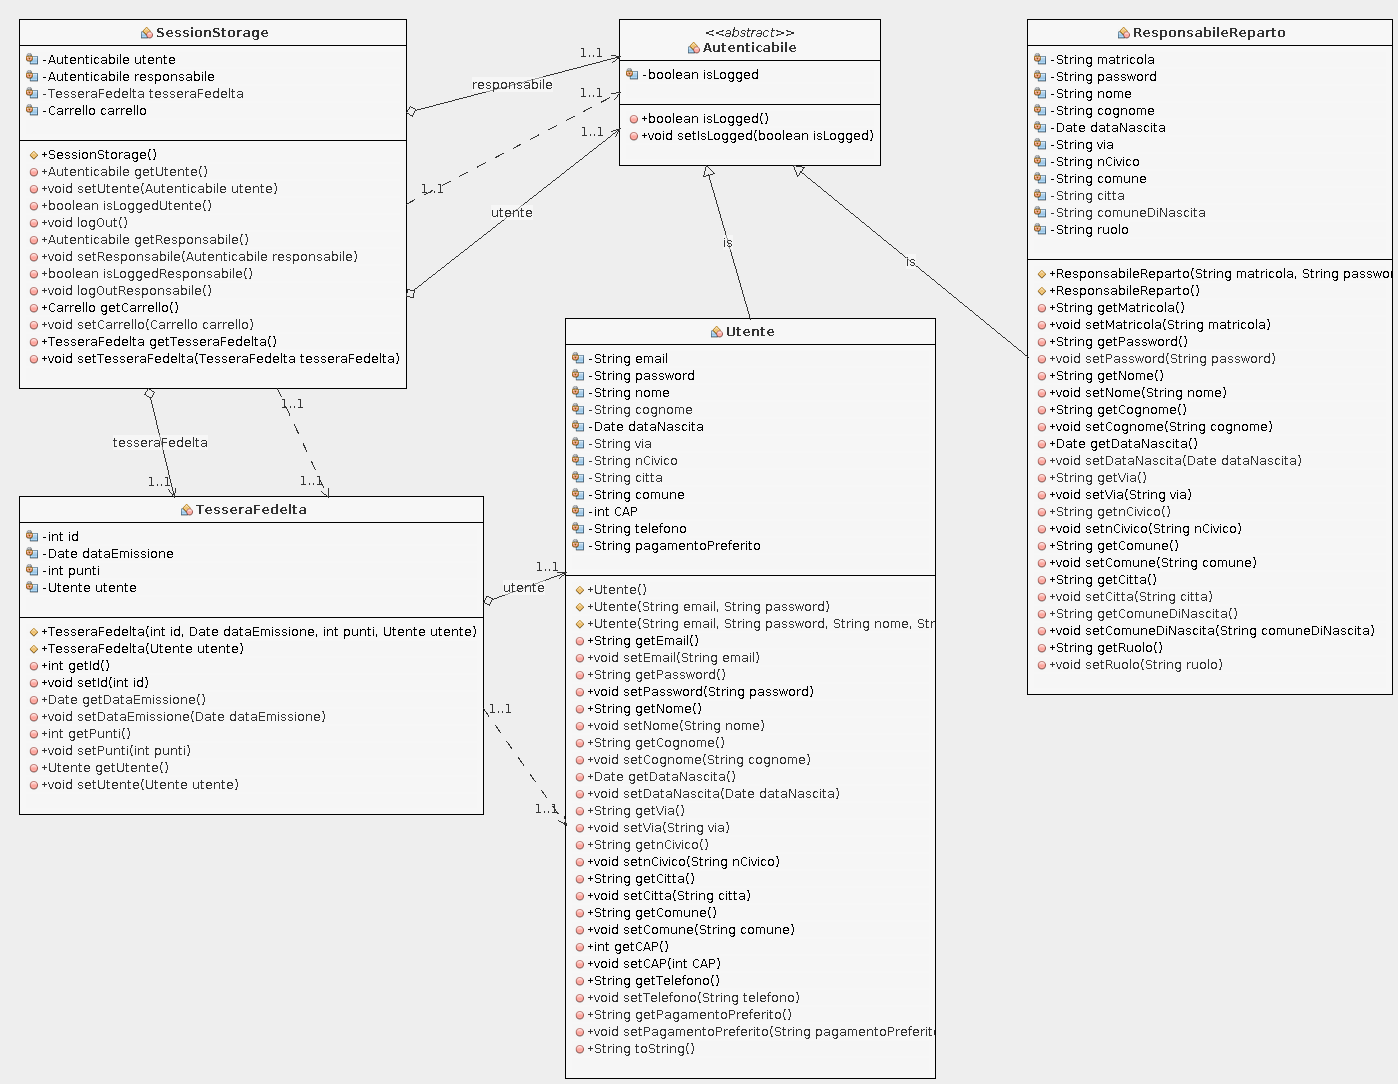
\includegraphics[width=\textwidth]{UmlAutenticabile.png}
	\caption{UML della classi Autenticabile, utente e responsabile.}
	\label{fig:UmlAutenticabile}
\end{figure}
Qui sono stati riportati vengono riportati i class diagram dei file fxml utilizzati nella View e dei relativi controller.
\begin{figure}[h!]
	\centering
	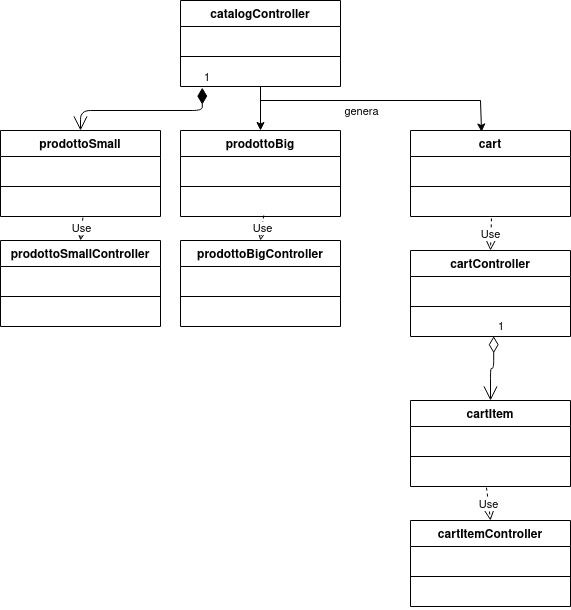
\includegraphics[width=\textwidth]{UmlCatalog.jpg}
	\caption{UML delle classi della vista Catalogo}
	\label{fig:UmlCatalog}
\end{figure}

\begin{figure}[h!]
	\centering
	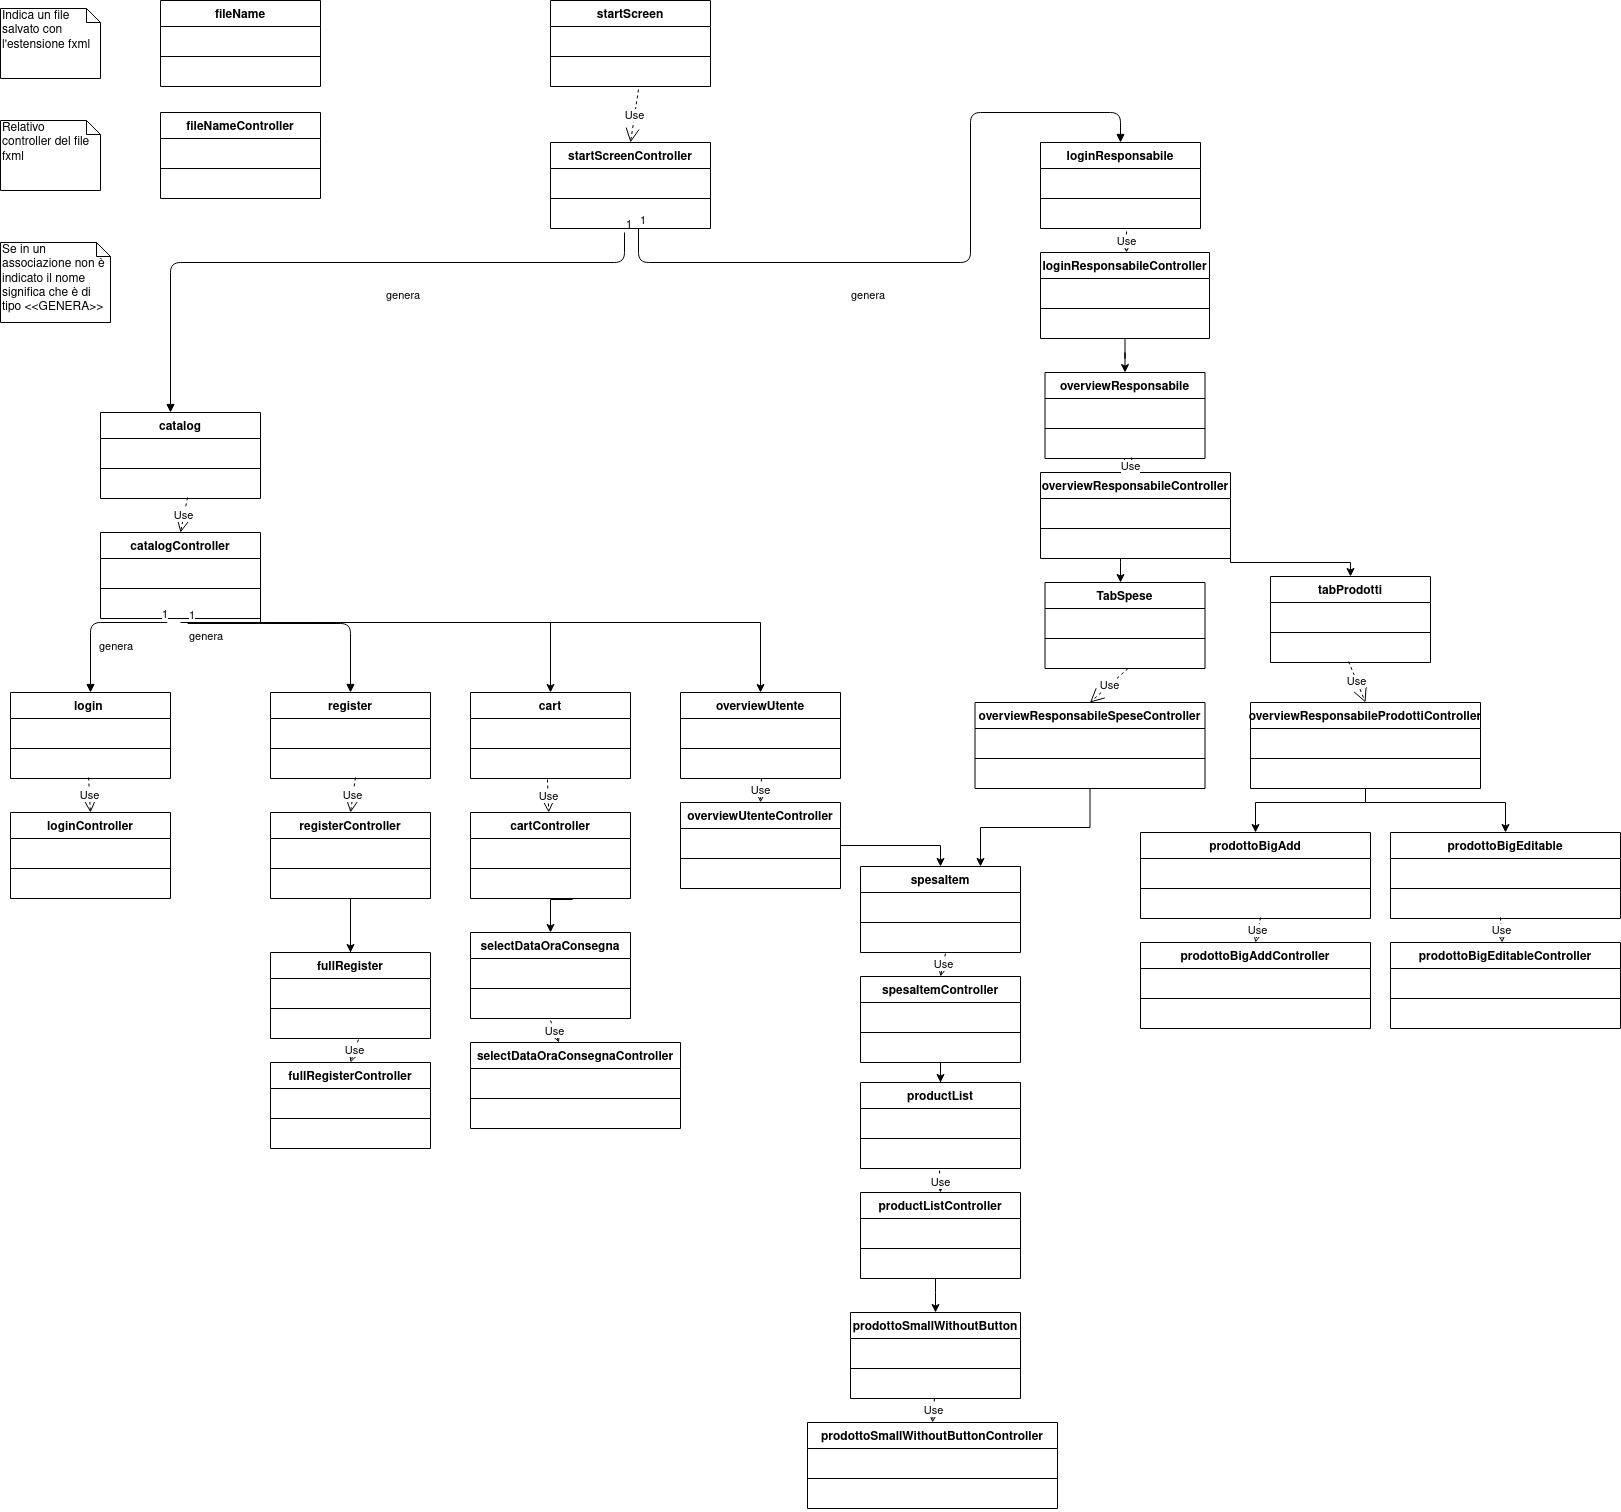
\includegraphics[width=\textwidth]{UmlInterfaccie.jpg}
	\caption{UML delle Classi di tutte le viste}
	\label{fig:UmlInterfaccie}
\end{figure}

\clearpage
\subsection{Diagrammi di sequenza del software implementato.}
Sono state inseriti di diagrammi di sequenza delle parti di software più significative e complesse e la parte di interfacce di responsabile reparto non è stata inserita perché risulta più semplice rispetto a quelle inserite.
\begin{figure}[h!]
	\centering
	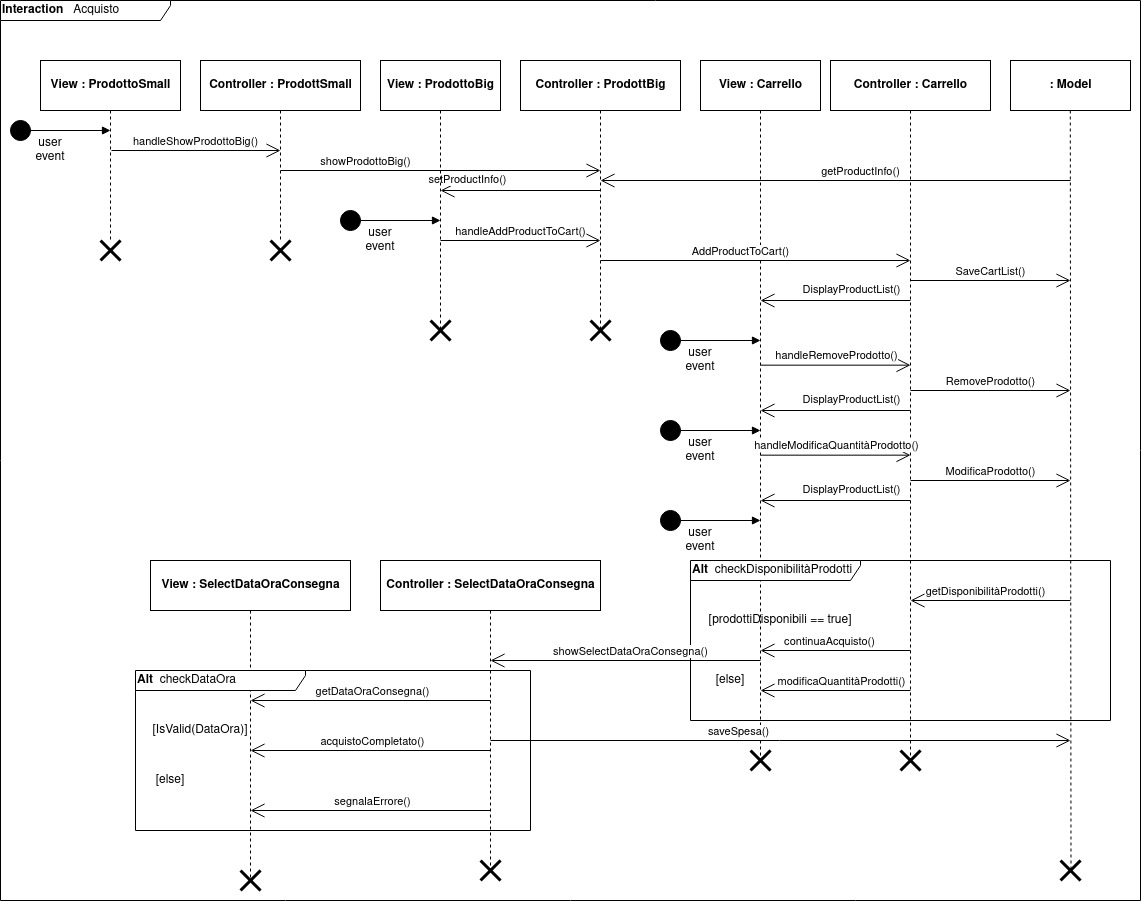
\includegraphics[width=\textwidth]{SDAcquisto.jpg}
	\caption{Diagramma di sequenza di un acquisto.}
	\label{SDAcquisto.jpg}
	\newpage
\end{figure}
\begin{figure}[h!]
	\centering
	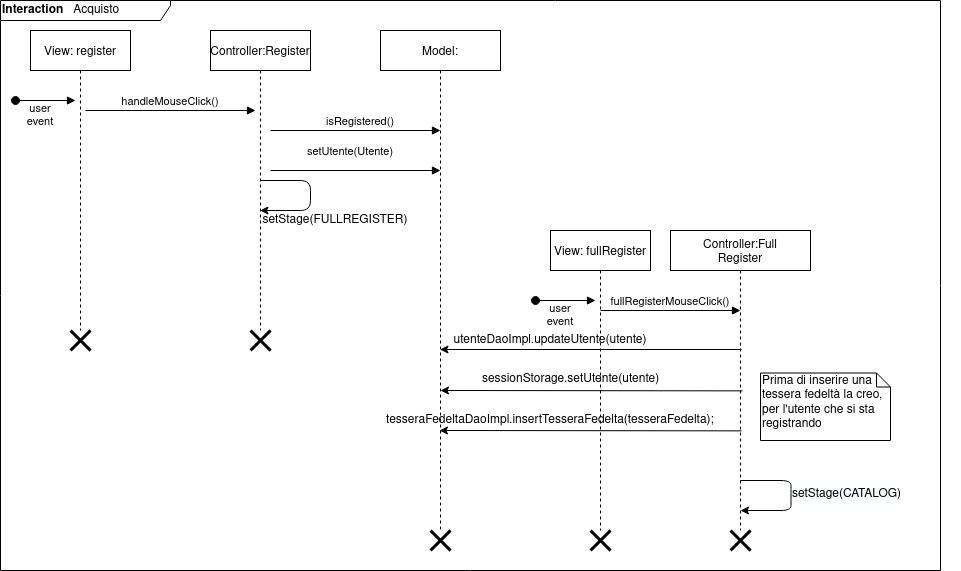
\includegraphics[width=\textwidth]{SequenceDiagramRegistrazione.jpg}
	\caption{Sequence Diagram della registrazione.}
	\label{fig:SequenceDiagramRegistrazione}
\end{figure}

\begin{figure}[h!]
	\centering
	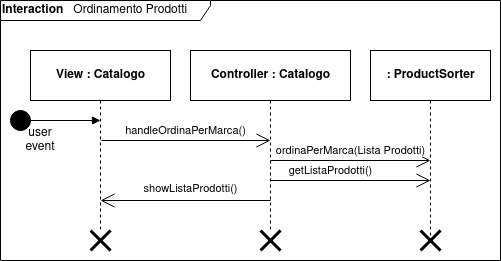
\includegraphics[width=\textwidth]{SDSorting.jpg}
	\caption{Diagramma di sequenza dell'ordinamento dei prodotti per marca}
	\label{fig:SDSorting}
\end{figure}

\clearpage
\subsection{Persistenza dati con Database SQL}
Utilizzare un database ha portato i seguenti vantaggi:
\begin{itemize}
	\item{
	      L'applicativo può utilizzare un qualsiasi database remoto specificando l'indirizzo e le credenziali d'accesso.}

	\item{
	      Possibilità di utilizza più istanze contemporaneamente dell'applicativo affidando la gestione
	      della concorrenza al DBMS.}
	\item{
	      Accesso e modifica dei dati facilitato con l'utilizzo delle interrogazioni.}
\end{itemize}


\noindent \`E stato utilizzato un database relazione e come DBMS MariaDB (fork open source di MySql),
per implementare la connessione si utilizza \textbf{JDBC}.
\newpage
\begin{lstlisting}[language = Java , frame = trBL , firstnumber = last , escapeinside={(*@}{@*)}]
    private static ConnectionDb instance = new ConnectionDb();
    private String url = "jdbc:mysql://localhost:3306/";
    private String dbname = "Spesa";
    private String username = "spesa";
    private String password = "spesa";
    private String multipleQueries = "?allowMultiQueries=true";
    private Connection connection = null;
    private Statement statement = null;
    private PreparedStatement pstmt = null;
    private ResultSet resultSet = null;

    private ConnectionDb() {
    }

    public static ConnectionDb getInstance() {
        return instance;
    }

    public PreparedStatement getPreparedStatement(String query) throws SQLException {
        this.connection = DriverManager.getConnection(url + dbname, username, password);
        this.pstmt = connection.prepareStatement(query);
        return pstmt;
    }

    public void doQuery(String query) throws SQLException {
        this.connection = DriverManager.getConnection(url + dbname + multipleQueries, username, password);
        this.statement = connection.createStatement();
        this.resultSet = statement.executeQuery(query);
        connection.close();
    }

    public int doSpecificQuery(String query) throws SQLException {
        this.connection = DriverManager.getConnection(url + dbname + multipleQueries, username, password);
        this.statement = connection.createStatement(java.sql.ResultSet.TYPE_FORWARD_ONLY,
                java.sql.ResultSet.CONCUR_UPDATABLE);
        this.statement.executeUpdate(query, Statement.RETURN_GENERATED_KEYS);
        int id = -1;
        this.resultSet = this.statement.getGeneratedKeys();
        if (resultSet.next()) {
            id = resultSet.getInt(1);
        }
        return id;
    }

    public ResultSet getResultSet() {
        return resultSet;
    }
\end{lstlisting}
\subsubsection{InitDb}
\noindent Implementazione di una classe di InitDb, utilizzata per creare e riempire le tabelle del
database. \`E stata creata un classe per ogni tabella presente nel database.
\begin{lstlisting}[language = Java , frame = trBL , firstnumber = last , escapeinside={(*@}{@*)}]
public class InitReparto {

    private ConnectionDb db;

    public InitReparto() {
        db = ConnectionDb.getInstance();
    }

    public void createReparto() throws SQLException {
        db.doQuery("CREATE TABLE `Reparto` (\n"
                + "  `nome` varchar(100) NOT NULL,\n"
                + "  PRIMARY KEY (`nome`)) ENGINE=InnoDB");
    }

    public void fillTableReparto() throws SQLException {
        db.doQuery("INSERT INTO `Reparto` (`nome`) VALUES "
                + "('Panetteria'),"
                + "('Pasticceria'),"
                + "('Pastificio'),"
                + "('Sughi e Salse'),"
                + "('Latteria'),"
                + "('Macelleria'),"
                + "('Pescheria'),"
                + "('Gastronomia'),"
                + "('Surgelati'),"
                + "('Frutta'),"
                + "('Verdura'),"
                + "('Bevande'),"
                + "('Vini e Liquori'),"
                + "('Oli e aceti'),"
                + "('Scatolame');");
    }
}
\end{lstlisting}
\newpage
\subsubsection{Diagramma ER}
\begin{figure}[h!]
	\centering
	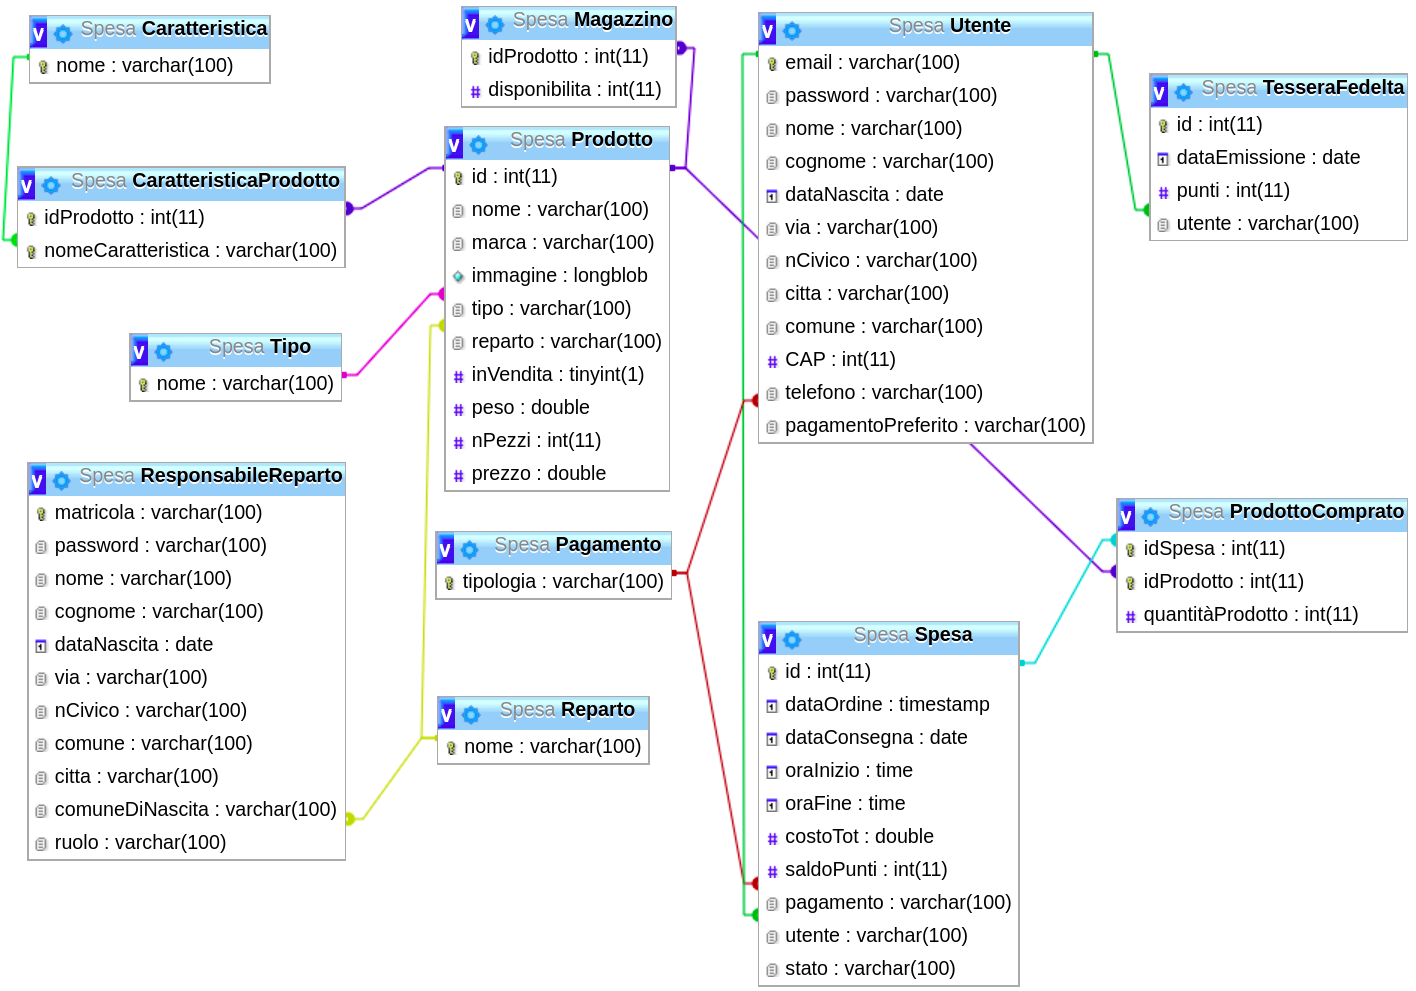
\includegraphics[width=\textwidth]{DiagrammaER.png}
	\caption{Diagramma Entity Relationship}
	\label{fig:DiagrammaER}
\end{figure}
\newpage
\subsection{Sicurezza}
Le password per l'autenticazione dell'utente e del responsabile reparto, per semplicità, sono state salvate in chiaro sul database.
Per un'evoluzione del prototipo si suggerisce di sostituire il testo delle password con un salted hash.
L'applicativo potrebbe essere vulnerabile ad attacchi di tipo SQL-injection poiché non è stato implementato alcun controllo per sopperire a questa eventualità.

\section{Attività di test e validazione}
Per verificare la solidità del prototipo prodotto, sono state effettuate le seguenti attività:
\begin{itemize}
    \item{Verifica della correttezza dei diagrammi rispetto al documento delle specifiche}
    \item{Controllo di consistenza tra diagrammi e codice}
    \item{Test di unità generici }
    \item{Test degli sviluppatori sul prototipo di software }
    \item{Test utente generico sul prototipo di software}
\end{itemize}
\subsection{Ispezione codice e documentazione}
\noindent
In questa fase è stato effettuato un confronto dei use case diagram con  il documento delle specifiche. Successivamente si è passati a produrre i sequence diagram relativi ai use case.
Sulla base della documentazione prodotta è stato sviluppato il codice da cui in seguito sono stati generati i diagrammi delle classi. Infine dopo aver accertato l'uso corretto dei pattern pensati durante la fase di progettazione, è stata fatta una nuova ispezione per trovare infrazioni o mancanze all'interno del codice.
\subsection{Unit test}
Durante questa fase è stata creata una versione alternativa del codice per valutarne il corretto funzionamento. E' stato fatto un test delle classi che presentavano funzionalità più complesse  e per verificare che i dati fossero inseriti correttamente all'interno del database.

\begin{lstlisting}[language = Java , frame = trBL , firstnumber = last , escapeinside={(*@}{@*)}]
import java.sql.Date;
import java.sql.SQLException;
import java.util.List;
import univr.spesaonline.model.Prodotto;
import univr.spesaonline.model.ProdottoDaoImpl;
import univr.spesaonline.model.Utente;
import univr.spesaonline.model.UtenteDaoImpl;

public class TestRunner {
    public static void main(String[] args) throws SQLException {
       Prodotto prodotto;
        List<Prodotto> prodotti;
        ProdottoDaoImpl prodottoDaoImpl;

        prodottoDaoImpl = new ProdottoDaoImpl();

        prodotto = new Prodotto(0, "Mele", "PinkLady", null, "Frutta", "Frutta", true, 1000, 10, 1.75);

        //inserimento prodotto 
        prodottoDaoImpl.insertProdotto(prodotto);
        prodotti = prodottoDaoImpl.getAllProdotto();
        //controllo inserimeto
        for (Prodotto p : prodotti) {
            if (p.equals(prodotto)) {
                System.out.println("Prodotto inserito");
            }
        }

        //modifica prodotto
        prodotto.setPrezzo(3.0);
        prodottoDaoImpl.updateProdotto(prodotto);
        prodotti = prodottoDaoImpl.getAllProdotto();
        //controllo modifica
        for (Prodotto p : prodotti) {
            if (p.equals(prodotto)) {
                System.out.println("Prodotto modificato");
            }
        }
        //inserimento di un utente
        Utente u;
        List <Utente> utenti ;
        UtenteDaoImpl utenteDaoImpl = new UtenteDaoImpl();
       
        Date date = Date.valueOf("1989-03-31");
        u = new Utente("b.rosi@gmail.com", "Ciao12", "Bianca","Rosi", date , "Via De Gasperi", "15","Verona", "Verona", 37030, "045521982","Paypal");
        utenteDaoImpl.register(u.getEmail(), u.getPassword());
        utenteDaoImpl.updateUtente(u);
        if(u.equals(utenteDaoImpl.login(u.getEmail(), u.getPassword())))
              System.out.println("Utente aggiunto nel db");
        
    }
    \end{lstlisting}
\subsection{Test degli sviluppatori}
Durante questa fase si è cercato di verificare il corretto funzionamento del sistema sia con input corretti che errati. In particolare le attività di test sono state suddivise in :
\begin{itemize}
    \item Inserimento di dati errati (ovvero che non rispettavano un certo pattern soprattutto per le stringhe come CAP o numero di telefono) o vuoti. 
    \item Inserimento di numeri negativi per esempio per il peso, il prezzo e la quantità di un prodotto inserito nel catalogo oppure dentro il carrello.
    \item Verifica della reazione del sistema con l'inserimento di duplicati come ad esempio la registrazione di nuovi utenti nel sistema con email già presente nella base di dati.
    \item Inserimento di un nuovo prodotto: è stato verificato se dopo l'inserimento di un nuovo prodotto da parte del responsabile reparto, il sistema dopo la pressione del pulsante di refresh mostra correttamente tutti i prodotti di quel reparto con il nuovo prodotto aggiunto.
    \item Registrazione di un nuovo utente: Controllo della email, password creata e successivamente un controllo sui dati anagrafici soprattutto sulla data di nascita che non può avvenire nel futuro e l'utente che si registra deve aver compiuto almeno diciotto anni per poter registrarsi.Questo ultimo vincolo è stato imposto per evitare il caso in cui utenti minorenni avessero provato ad acquistare alcolici.
    \item Verifica data e orario di consegna della spesa: i controlli sono stati fatti sulla data di consegna che può avvenire nei sette giorni successivi alla data attuale in cui l'utente conferma la spesa, sull'ora di inizio e fine della consegna (l'ora di fine non può avvenire prima dell' ora di inizio e l'ora di inizio e fine non può essere uguali).
    \item Verifica dell'aggiunta di una nuova spesa all'elenco delle spese effettuate da parte dell'utente e all'elenco di spese visibile ai responsabili reparto. 
    \item Controllo dello svuotamento del carrello dopo che l'utente ha confermato la spesa
    \item Controllo della disponibilità dei prodotti al momento della conferma della spesa
    \item Verifica dell'aggiornamento dei dati dopo la modifica di un prodotto o del profilo di un utente.
    \item Verifica del login di utente e responsabile reparto. In aggiunta per l'utente il controllo su log out.
    \item Verifica del corretto funzionamento del cambio di interfacce e dei pulsanti
    \item Verifica che l'interfaccia visibile dall'utente se non autenticato premetta la visione del catalogo dei prodotti e del carrello. Mentre se l'utente ha effettuato il login deve visualizzare in più anche i pulsanti per vedere le informazioni dell'utente e non mostrare invece quelli di login e di registrazione.
    \item Controllo se durante la pressione del pulsante acquista il sistema verifica se l'utente è già autenticato e se non lo è, gli che gli venga mostrata la schermata di login.
    \item Verificato che il sistema impedisse l'acquisto di un carrello senza prodotti.
    \item Verifica della consistenza dei dati inseriti come prova all'interno della base di dati.
\end{itemize}
\subsection{Test utente generico}
Come ultimo passo il prototipo è stato sottoposto a un test di utilizzo da parte di persone con limitata conoscenza informatica al fine di far emergere eventuali errori o bug presenti che non sono stati esaminati dagli sviluppatori. Gli utenti non sono stati guidati passo passo nell'utilizzo di questo software soprattutto per non influenzare l'andamento del test. Si è data solo una breve spiegazione dello scopo del software e dell'uso. In conclusione gli utenti generici hanno dato dei consigli preziosi su come migliorare il software sia in termini di usabilità (per rendere il software ancora più user-friendly e intuitivo) sia per nuove funzionalità da aggiungere per rendere il prototipo più completo.
\end{document}
